%-----------------------------------------------------------------
%	DINÀMICA MOL·LECULAR
%	!TEX root = ./../main.tex
%-----------------------------------------------------------------
\section{Dinàmica molecular}
La dinàmica molecular consisteix en estudiar explícitament l'evolució temporal de les partícules (molècules) segons les lleis de la mecànica clàssica.

Les fonts d'aleatorietat estan en:
\begin{itemize}
	\item Les condicions inicials, com ara les posicions inicials.
	\item L'estadística que segueixen les partícules (i.e., clàssica, o quàntiques) per determinar les velocitats inicials.
\end{itemize}
Cada simulació és diferent, i el que ens interessa és estudiar el comportament mitjà.

\begin{example}\label{ex:temperature}
	Volem determinar la temperatura del sistema (variable macroscòpica). De la mecànica estadística sabem que
	\begin{flalign*}
		\ev{\frac{1}{2} m v^{2}} &= \frac{1}{2} k_{B} T \Rightarrow T = \frac{m}{k_{B}} \ev*{v^{2}} = \frac{m}{k_{B}} \frac{1}{N} \sum_{i=1}^{N} v_{i}^{2}. &
	\end{flalign*}
	Pel que fa a l'error del càlcul de $T$ hauríem de tenir en compte les fluctuacions de $v$. El que ens interessa és treballar en el límit termodinàmic ($N \to \infty$), ja que $\Delta T \propto N^{-1/2}$.
\end{example}

\subsection{Algoritme bàsic d'un programa de dinàmica molecular}
\begin{enumerate}[i)]
	\item Llegir els \emph{inputs} d'entrada (e.g., $T$, $N$, etc.)
	\item Inicialitzar $\va{x}_{i}$, $\va{v}_{i}$ (posicions i velocitats).
	\item Computar les interaccions entre partícules, $\va{F}_{ij}$ (força entre la partícula $i$-èssima i $j$-èssima).
	\item Es fa evolucionar $\va{x}_{i}$, $\va{v}_{i}$ d'acord amb les lleis de la mecànica clàssica.
	\item Repetir els passos i)--iv) fins arribar a un temps determinat.
\end{enumerate}

\subsubsection*{Com inicialitzar $\va{x}_{i}$, $\va{v}_{i}$?}
Típicament $\va{x}_{i}$ està distribuïda uniformement en tot el domini (això es pot aconseguir amb un nombre aleatori que segueixi una distribució uniforme).

Altrament, típicament $\va{v}_{i}$ segueix una distribució de Maxwell-Boltzmann (cada component de $\va{v}_{i}$ és una variable gaussiana independent de les altres). Per poder fer això podem emprar el mètode de Box--Muller.

\begin{meth}[de Box--Muller]\label{met:box-muller}
	Donades dues variables aleatòries $U_{1}$ i $U_{2}$ distribuïdes uniformement en $(0,1)$, aleshores podem definir dues variables
	\begin{align}
		Z_{1} = \sqrt{-2 \ln U_{1}} \sin (2\pi U_{2}) \qc Z_{2} = \sqrt{-2 \ln U_{1}} \cos (2\pi U_{2})
	\end{align}
	que són dues variables aleatòries gaussianes amb mitjana $\mu = 0$ i $\sigma = 1$.
\end{meth}

\subsubsection*{Com computar $\va{F}_{ij}$?}
Calcular totes les parelles $\va{F}_{ij}$ farà que el temps de computació sigui proporcional a $N (N-1)/2 \sim N^{2}$. Com que ens interessa simular en el límit de termodinàmic, cal reduir aquesta dependència, cosa que podem fer emprant una llista de Verlet.
\begin{meth}[Llista de Verlet]\label{meth:llista-verlet}
	Suposant que les interaccions només són fortes en un entorn $\mc{E}\sast(\va{r}_{i},r_{v})$, podem agafar un entorn més gran $\mc{E}\sast(\va{r}_{i},r_{c} > r_{v})$ i computar totes les interaccions de la partícula $i$ amb totes les de l'interior de $\mc{E}\sast(\va{r}_{i},r_{c})$, de manera que el temps en què les partícules llistades per fer el càlcul d'interaccions serà superior.
	\begin{figure}[H]
		\centering
		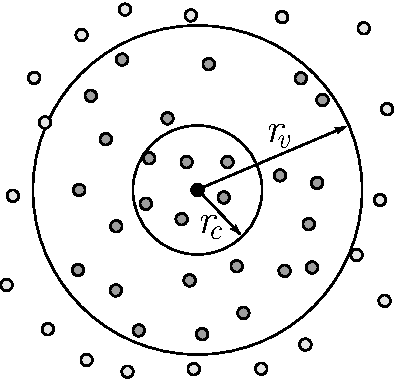
\includegraphics[width=0.3\textwidth]{./images/llista-verlet}
		\caption{Representació gràfica de la llista de Verlet}
		\label{fig:llista-verlet}
	\end{figure}

	Ara cada pas de temps de computació de les interaccions és proporcional a $N$, i de tant en tant cal actualitzar la llista (amb $t \propto N^{2}$). En global reduïm el temps de computació a $\propto N^{3/2}$.
\end{meth}

\subsubsection*{Com fer evolucionar $\va{x}_{i}$, $\va{v}_{i}$?}
Necessitem discretitzar les lleis de la mecànica clàssica. Per això podem emprar l'algoritme de Verlet.

\begin{meth}[Algoritme de Verlet]\label{meth:algoritme-verlet}
	Típicament, podem calcular l'evolució de la posició emprant un desenvolupament de Taylor:
	\begin{flalign*}
		\va{r}_{i}(t \pm \Delta t) &= \va{r}_{i}(t + \Delta t) \pm \pdv{\va{r}_{i}(t)}{t} \Delta t + \pdv[2]{\va{r}_{i}(t)}{t} \Delta t^{2} + \order{\Delta t^{3}} & \\
		&= \va{r}_{i}(t) \pm \va{v}_{i}(t) \Delta t + \frac{\va{F}_{i}(t)}{2m} \Delta t^{2} + \order{\Delta t^{3}}
	\end{flalign*}
	on $\va{F}_{i} = \sum_{j=1}^{N-1} \va{F}_{ij}$.
	Així doncs, trobem una expressió per a $\va{r}_{i}(t + \Delta t)$ més precisa (observem que passem de $\order{\Delta t^{3}}$ a $\order{\Delta t^{4}}$) i que no requereix el còmput de la velocitat:
	\begin{align}
		\va{r}_{i}(t + \Delta t) = 2 \va{r}_{i}(t) - \va{r}_{i}(t - \Delta t) + \frac{\va{F}_{i}(t)}{m} \Delta t^{2} + \order{\Delta t^{4}} &
	\end{align}
\end{meth}

\subsubsection*{Com computar les variables macroscòpiques?}
A l'exemple~\ref{ex:temperature} hem vist com calcular la temperatura a partir de les velocitats de les partícules. Ara veurem com calcular la pressió.

\begin{example}
	La pressió d'un gas ve donada per l'intercanvi de moment de les partícules amb les parets.
	\begin{figure}[H]
		\centering
		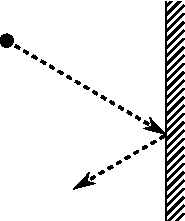
\includegraphics[width=0.15\textwidth]{./images/xoc-elastic}
		\caption{Xoc elàstic d'una partícula amb una paret}
		\label{fig:xoc-elastic}
	\end{figure}
	En el cas d'una variació de moment unidimensional en un xoc elàstic (figura \ref{fig:xoc-elastic}), el que tenim és
	\begin{flalign*}
		% \abs{P} &= \abs{\frac{F}{A}}_{\text{xocs}} = \frac{1}{A_{\text{paret}}} \abs{\frac{\Delta p}{\Delta t}}_{\text{xocs}} \approx \frac{1}{A_{p} \Delta t} \abs{\Delta p}_{\text{xocs}} = \frac{1}{A_{p} \Delta t} \abs{\Delta p_{y}}_{\text{xocs}} = \frac{2m}{A_{p} \Delta t} \abs{\Delta v_{y}} &
		\abs{P} &= \abs{\frac{F}{A}}_{\text{xocs}} = \frac{1}{A_{\text{paret}}} \abs{\frac{\Delta p}{\Delta t}}_{\text{xocs}} \approx \frac{1}{A_{p} \Delta t} \abs{\Delta p}_{\text{xocs}} = \frac{1}{A_{p} \Delta t} \abs{p_{y}}_{\text{xocs}} = \frac{2m}{A_{p} \Delta t} \abs{v_{y}} &
	\end{flalign*}
	on $\Delta t$ és un pas de temps. Cal observar que per a un pas de temps $\Delta t$ molt petit, la quantitat de xocs que es produeixin a cada pas fluctuaran molt i, per tant, el valor de la pressió (figura \ref{fig:fluct-pressio}). Així doncs, el que caldria seria calcular $\ev{P}$ (comportant més càlculs), o bé augmentar $\Delta t$ (comportant una reducció en la precisió).
	\begin{figure}[H]
		\centering
		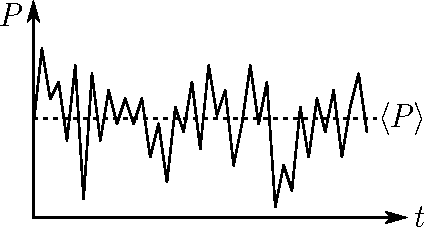
\includegraphics[width=0.35\textwidth]{./images/fluct-pressio}
		\caption{Fluctuacions en el càlcul del valor de la pressió}
		\label{fig:fluct-pressio}
	\end{figure}
\end{example}

\subsubsection*{Aspectes a considerar en implementar un algoritme de dinàmica molecular}
En un algoritme de dinàmica molecular, és important trobar un equilibri entre els tres aspectes següents:
\begin{itemize}
	\item La velocitat de l'algoritme.
	\item La precisió de l'algoritme ($\sim \Delta t^{-1}$).
	\item El requeriment de memòria de l'algoritme.
\end{itemize}

\begin{thm}[Inestabilitat de Lyapunov]
	Dues trajectòries que difereixen en la seva condició inicial comporta, al cap del temps, una distància entre elles que creix exponencialment.
\end{thm}

Un altre factor que hauríem de tenir en compte és la inestabilitat de Lyapunov. Tot i que una variació en les condicions inicials comporta un canvi en el resultat final d'una simulació, a priori, el comportament mitjà serà independent de la tria de les condicions inicials.
